\section{Aufbau}
\label{sec:Aufbau}

Wie in Abbildung \ref{fig:abb} zu sehen, besteht das Experiment aus zwei Helmholtz-Spulen, die das externe magnetische Feld erzeugen und zwischen denen eine Haltung für eine Kugel angebracht ist. Mithilfe eines Luftkissens kann sich diese reibungsfrei bewegen.\newline
Die als Vollkugel zu nähernde Billardkugel besitzt einen Permanentmagneten in ihrem Inneren und einen Stiel zur Halterung für eine als masselos angenommene Aluminiumstange. Auf diese kann eine Punktmasse aufgesteckt und frei bewegt werden.\newline
An der oberen Helmholtz-Spule ist außerdem ein Stroboskop angebracht.
Mit dem Steuerungsgerät lassen sich die Stromstärke für das Magnetfeld der Helmholtz-Spulen, das Stroboskop und das Luftkissen einstellen.

\begin{figure}
\centering
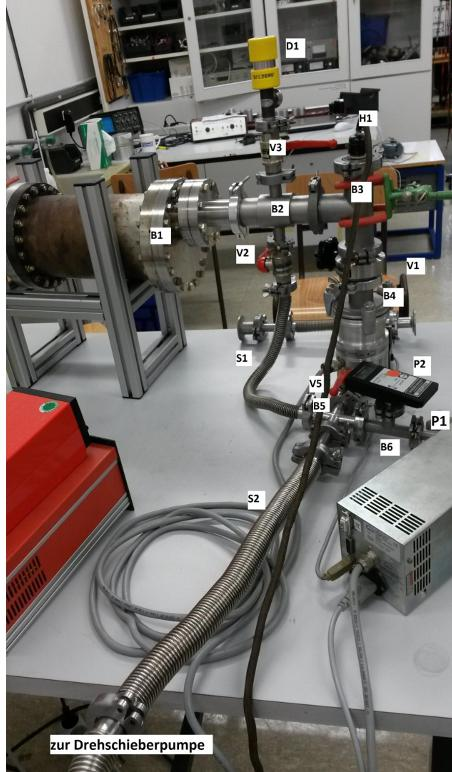
\includegraphics[scale = 0.5,keepaspectratio]
	{content/images/Aufbau.eps}
\caption{Aufbau des Versuchs zur Bestimmung des magnetischen Moments\cite{V105}}
\label{fig:abb}
\end{figure}